\begin{scanpage}{0208}{190}
\noindent is its field on the conductor surface, where the external currents $\mathbf j_2^m$ are specified; $\mathbf E_2$ is the field created by these currents at point 1 (Figure 74).
\par\medskip\noindent\begin{minipage}[t]{.43\linewidth}\vspace{0pt}
\centering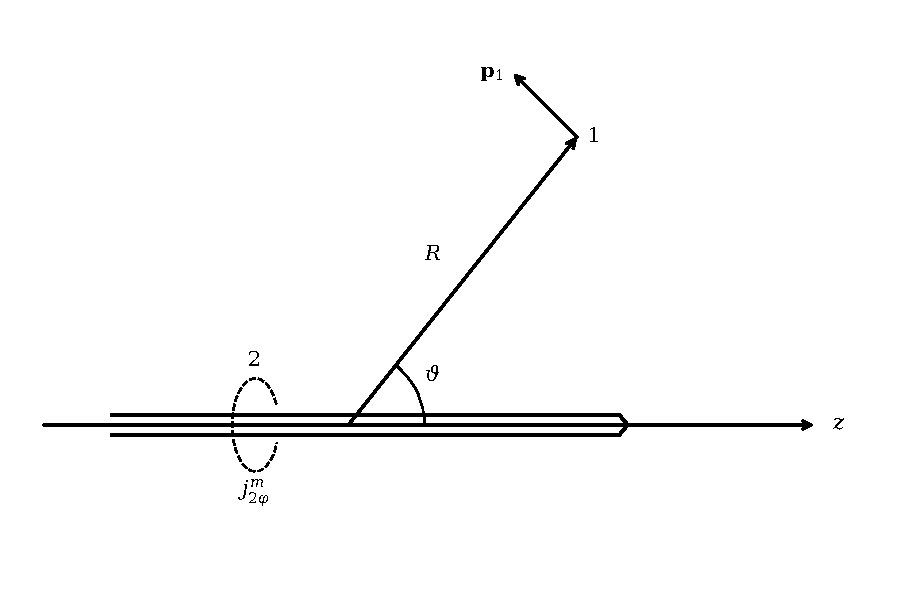
\includegraphics[width=.95\linewidth]{images/recreated/r-0208-fig74.pdf}\par Figure 74.
\end{minipage}\hfill\begin{minipage}[t]{.53\linewidth}\vspace{0pt}
The external current $\mathbf j_2^m$ is determined by the well-known equation
\[\mathbf j_2^m=-\frac{c}{4\pi}[\mathbf n\mathbf E]\tag{30.20}\]
in terms of the electric field $\mathbf E$ on the conductor's surface. In view of the boundary condition
\[E_z+E_z^e=0\tag{30.21}\]
\end{minipage}\par\medskip
\noindent we have
\[j_{2\varphi}^m=-\frac{c}{4\pi}E_z^e.\tag{30.22}\]
Furthermore, defining the dipole moment $p_1$ in terms of its field in free space (at the point $x=y=z=0$)
\[E'_{0z}=-k^2p_1\frac{e^{ikR}}R\sin\vartheta\tag{30.23}\]
and changing from the magnetic intensity $H_{1\varphi}$ to the total current
\[J=\frac{ca}2H_{1\varphi},\tag{30.24}\]
induced by the dipole in the conductor, we obtain from the Lorentz lemma the following relationship:
\[E_{2\vartheta}=H_{2\varphi}=\frac{k^2\sin\vartheta}{i\omega E'_{0z}}\cdot\frac{e^{ikR}}R\cdot\int_{-\infty}^{z_2}E_z^eJ(z)\,dz.\tag{30.25}\]
If the dipole $\mathbf p_1$ is moved to a distance $R\gg z_2-z_0$, then the field radiated by it may be investigated on the section $z_2-z_0$ of
\end{scanpage}
